% Hauptdatei der Vorlage fuer Seminararbeiten am Lehrstuhl f{\"u}r Hochleistungsrechnen (nicht ver{\"a}ndern!)
% Veraenderungen bitte ausschliesslich in den (an den mit "HIER": 
% gekennzeichnenten Stellen) eingebundenen Dateien vornehmen

\documentclass[10pt,          % Schriftgroesse einstellen
               a4paper,       % Seitenformat w{\"a}hlen
               twocolumn,     % zweispaltiges Layout
               DIV14,         % Groesse des Satzspiegels (Warnung dazu bitte ignorieren!)
               BCOR=8mm,      % Bindekorrektur (abgestimmt auf LfBS-Bindeger{\"a}t)
               twoside        % Beidseitiger Druck
               %abstract=true, % Titel des Abstract ausgeben
              ]{scrartcl}
\usepackage{hpcseminar}
\usepackage[english]{babel}   % HIER: Im Falle des Falles "english"
\usepackage[utf8]{inputenc}  % UTF-8 (viele aktuelle Editoren unter Linux, Mac und Windows)

\usepackage[T1]{fontenc}      % u.a. Richtige Worttrennung
\usepackage{lmodern}          % Verbesserte "Computer Modern"-Schriften laden
\usepackage{graphicx}         % Grafiken einbinden
\usepackage{units}            % Einheiten setzen mit z.B. \unit[10]{MB} und \unitfrac[100]{Mbit}{s}
\usepackage[binary-units = true]{siunitx}         % Wesentlich umfangreicheres Einheiten Paket als Ersatz f{\"u}r "units"

% In dieser Datei koennen eigene Erweiterungen eingebracht werden
% HIER: Nur wenn n{\"o}tig Datei my_includes.tex aendern
\usepackage{caption}
\usepackage{nameref}
\newcommand{\source}[1]{\caption*{Source: {#1}} }



%% Beginn des eigentlichen Dokumentes
%%-----------------------------------
\begin{document}

%% Ein paar wichtige Details konfigurieren
%% Ein paar wichtige Details konfigurieren
%%----------------------------------------
\title{Titel der Seminararbeit}
\author{André Merboldt}
\betreuer{Dipl.-Inf. Vorname Nachname}
\semester{Wintersemester 2015/2016}
\keywords{CUDA, optimization, synchronization, memory, unified memory}


% Titel automatisch erzeugen
\maketitle

% Abstract
\begin{abstract}
Following the increasing demand for faster compputation, we will discuss various techniques of the CUDA Runtime and optimizations of memory transfer and access patterns.\\
While CPUs are able to maintain levels of performance, GPUs can achieve higher parallelism due to the parallel concept of graphics processing. Unlike CPUs, graphics units operate at a lower frequency, but have many more cores to make up for it.\\
In order to fully make use of the massive parallelism, we have to apply several techniques like coalescing access to global memory to achieve the highest possible throughput.\\

% Automatische formatierte Ausgabe der oben angegebenen Keywords
\keywordsline
\end{abstract}

% Hier werden die Kapitel eingebunden
% Bei Bedarf weitere Kapitel eintragen
\section{Introduction}
\label{sec:intro}
Performance optimizations of CUDA applications, or any high performance GPU computing program for that matter, can be roughly seperated into three sections.\\
First, increasing instruction usage to maximize instruction troughput.\\
Secondly, utilize the GPU hardware to its full extent by maximizing parallelized execution.\\
While touching parts of the second section, we will focus our optimizating efforts on the third section (? other word), 
optimizing the memory transfer and access to achieve the highest possible memory throughput/bandwidth(?).\\
\\
In the first two chapters we will briefly outline (double?) the CUDA library, hardware architecture and the CUDA memory management.\\
Then, the main topic of this paper will be highlighted: the optimization of memory transfer and access.\\
As both GPUs and CUDA itself matured over time and CUDA is backwards-compatible, but not fordware-compatible,
focus will be on CUDA at version 7.5 and on devices of compute capability 2.x to 5.x.\\
%CUDA platform-independent and device-independent is an API by NVIDIA to utilize GPUs for accelerated computation.\\
%As both GPUs and CUDA itself matured over time, we will discuss CUDA at version 7.5 and highlight devices of compute capability 2.x to 5.x.\\
%To enable high performance computation, we have to efficiently pass data around and optimize access to memory.\\
%Prior to the discussion of optimization techniques, we will outline the basics of computation using GPUs with CUDA.

\section{Hardware Architecture}
\label{sec:hardware}
\subsection{Overview}
Each GPU contains several multiprocessors (current hardware up to 
In contrast to the more sequential CPU computational flow, GPUs work highly parallelized.

This parallelization is because of many more computational cores 

Due to GPU hardware having more cores than CPUs, computation is organized into threads which are meant to be executed in parallel, grouped into multiple \textbf{blocks}, called a \textbf{grid}. Both grids and threadblocks can have a dimension up to 3. Using these constructs, it is easily possible to index a multidimensional structure.\\
Grids are created upon a call of a \textbf{kernel} - that is a code sequence running on CUDA-capable devices - (?). Below is an illustrated overview of one two dimensional grid (3x3) of blocks each running a number of threads.\\
\begin{figure}
    \centering
    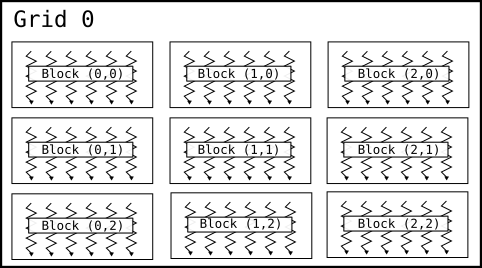
\includegraphics[scale=0.5]{media/threads_blocks_grid.png}
\end{figure}
\\
CUDA assigns blocks to streaming multiprocessors, 
\subsection{Memory}
\subsubsection{Device}
\paragraph{Global Memory}
\label{hardware_global}
The most ample of all GPU memory, often exceeding several gigabytes on current hardware, is accessible to all threads on the GPU and per PCIe even to the host.\\
Global memory is located off-chip, resulting in a higher latency around 500 clock cycles which is often hidden through thread parallelism but still a way higher bandwidth than the connection per PCI Express between host and device.\\
Memory transactions are used to global memory and these have to be aligned to their transaction size of 32, 64 or 128 bytes.\\
The high latency can impose a significant performance loss, to minimize its impact CUDA will try to merge as many transactions as possible. We will explore these coalescing mechanisms later in ~\ref{global_access}.\\
\paragraph{Shared Memory}
Due to being located on-chip, therefore resulting in low-latency, high-bandwidth memory, shared memory is used to exchange data between threads in a block and synchronize them.\\
Additionally shared memory is ideally suited to manually cache global memory.\\
\paragraph{Registers}
Data used without keywords (shared, global aka device) in a kernel are stored in registers, as long as they can hold it.\\
Though there are multiple thousands register (between 32K and 128K for current hardware) available for use by the compiler,
these registers have to be split between concurrently running threads on a multiprocessor.\\
Should the compiler decide that local data is too big to be hold in register only,
it will be stored in local memory which is by orders slower than registers or shared memory.\\
This phenomenon is called \emph{register pressure} and should be avoided by investigating local memory usage
and using shared memory.\\
\paragraph{Local Memory}
Contrary to its name is local memory not located on-chip, but in global memory.
Therefore it inherits its characteristics, most important the high latency which may limit an applications performance immensly.
To avoid local memory usage, the compiler supports a switch called \emph{--ptxas-options=-v} with which several information regarding
the generated code is shown. 
\paragraph{L1 Cache}
L1 Cache is on-chip memory, caching access to local memory. Shared memory and L1 cache are sharing the same memory space. \\
\paragraph{L2 Cache}
In contrast to L1 cache, L2 Cache is shared between all multiprocessors and is used to cache access to local and global memory.\\
% TODO: show when introduced etc.
\paragraph{Texture Memory \& Cache}
Texture memory can be used to hold data aswell and is optimized to store two dimensional data.\\
\subsubsection{Transfer}
GPUs are connected to a hostsystem via PCI Express, which limits the bandwidth of the memory transfer between host and device.\\
PCI Express is a point-to-point system (source?) and as data exchange is done using packets,
there is a significant overhead involved.\\
\begin{table*}
\centering
\begin{tabular}{c|c|c|c}
\textbf{Generation} &   \textbf{Transfer-Rate}      & \textbf{per Lane} & \textbf{16-lane}\\
\hline\hline
PCIe 1.0     &   2.5 GT/s               & 2 GBit/s          & 32 Gbit/s\\
PCIe 2.0     &   5.0 GT/s               & 4 GBit/s          & 64 GBit/s\\
PCIe 3.0     &   8.0 GT/s               & 7.87 GBit/s       & 126 Gbit/s\\
PCIe 4.0     &   16.0 GT/s              & 15.754 GBit/s     & 252 GBit/s\\
\hline
\end{tabular}
\caption{Comparison of different iterations of the PCI Express protocol, source: pcisig.com}
\label{tab:pci_comp}
\end{table*}
\emph{**show GPU Global memory transfer rates**}
As a comparision, GDDR5 (double rate type 5 synchronous graphics random access memory) is able to maintain a bandwith in excess over 100/200 GB/s.
\\
As we can see, the GPU memory is several times faster than the PCIe protocol theoretical maximum bandwidth.\\
This means we will have to try to minimize data transfer between host and device as PCIe is many times slower than device memory.
We will exploit this knowledge to achieve (?) high computational throughput (?).
\subsection{Kernel}
A \emph{Kernel} is a code procedure launched from the host and executed in a grid of threadblocks on the graphics unit.\\
Once the CUDA code is loaded onto the GPU, a global scheduler distributes the threadblocks to the streaming processors, in which then warp schedulers select 32 threads ( one warp ) for execution.\\

\section{Memory Management}
\label{sec:management}
\subsection{Memory Allocation}
\label{sec:mem_alloc}
We need to differentiate the allocation of host and device memory.
While we can allocate host memory using malloc, but not exclusively, device memory is generally allocated using cudaMalloc.
\emph{cudaMalloc()} can allocate a linear memory in the device memory, given the device has enough free memory.
Important to note is that \emph{cudaMalloc()} is always blocking, as an alternative can cudaMallocAsync be used which uses streams (...?).



Allocation and Deallocation are expensive operations and as a consequence we should reuse memory whereever it is possible.
(maybe show timings?)
\subsubsection{Dynamic Allocation}
Since compute capability 2.x, CUDA developers can allocate global memory in their kernels using \emph{malloc()} and operate using \emph{memset()} and \emph{memcpy()}.
\subsubsection{Pitched Layout}
Due to coalescing constrains, which we will discuss in depth in ~\ref{sec:access}, it is possible to allocate \emph{pitched memory}.\\
This memory is used for 2D and 3D memory, where the column or row number is not easily divided by a power of 2.\\
Therefore we can allocate this memory using a padding, where we use more memory than we need, but align the data in a way in which it is easily accessible.\\
Illustration:
\subsection{Streams and Synchronization}
\subsubsection{Synchronization}
In a highly parallized enviroment like CUDA, it is critical to synchronize the threads to allow benefitial collaboration.\\
CUDA provides several mechanics for developers to enable and simplify this process. CUDA applications has to synchronize on several depths, first on the threadblock level, where threads have to synchronize using shared memory and \_\_syncthreads() its work.\\
Secondly interblock synchronization can be implemented using cudaEventSynchronize() and \emph{cudaStreamSynchronize()}. Lastly (?), CUDA events may be used with \emph{cudaStreamWaitEvent()} to enable inter-GPU synchronization.\\
Additionally, there is the possibility to use atomic operations which are guaranteed to be "unteilbar"?? on device memory and are implemented by the graphics memory controller. 
\subsubsection{Streams}
\label{sec:streams}
Operations like memory copy or kernel launches are enqueued into a sequence, which is called a \emph{stream} in CUDA.\\
It is possible and often advantagous due to parallelized matters to use multiple streams which are able to run concurrently.\\
Using streams it is possible to implement for example overlapped data transfer.
\subsection{Unified Virtual Addressing}
\label{sec:uva}
Before the introduction of \emph{Unified Virtual Addressing} (UVA) in CUDA 4, address spaces of device and host were separate, which implied that every memory transfer has to specify which address space to target. (? expression)\\
UVA combines both address spaces to create a single unified virtual address space in which data from both device and host reside. This concept results in a simplified view of memory and enables the developer to stop using \texttt{cudaMemcpyDeviceToHost} and \texttt{|cudaMemcpyHostToDevice|} and use \texttt{cudaMemcpyDefault} in \emph{cudaMemcpy} methods.
Because of the unified address space, UVA only works on 64 bit operating systems, as 32 bit systems can only allocate roughly 4 GB and modern computers often exceed these limitations, especially combined with device memory.\\
UVA also enables \emph{Zero-Copy}~\ref{sec:zerocopy}.
\subsection{Unified Memory}
\label{sec:unified_memory}
\emph{Unified Memory}, introduced in CUDA 6, simplifies memory management with managed memory which is available to device and host equally.\\
With Unified Memory it is possible to allocate memory using \emph{cudaMallocManaged} and pass the pointer to a kernel, which is able to operate directly on it without the use of copies.

\section{Memory Transfer Optimization}
\label{sec:transfer}
\subsection{Pinned Memory}
One of the most important aspects of optimization is the memory transfer
from device and host ("und umgekehrt"/ and in reverse?).
As we have seen in "Hardware Spec" (figure pci), PCIe 2.0 has a theoretical bandwidth of 8 GB/s.
Unfortunely, this theoretical bandwidth is limited by several factors, most impactful the processor on the Host (? citation needed).
To bypass this limitation it is possible to \emph{pin host memory} to the device.\\
This means that we have direct memory access (DMA) to this memory (RAM).
The important bit of this technique is, that this pinned memory is page-locked, so it can't be swapped ( or even accessed??) by the host system.
As this method locks the CPU out of the equation (through DMA), we can achieve a bandwidth of 6 GB/s (in comparision to... GB/s with page-able memory)
The drawback of this method is the impact on the host system, as it can lower the systems performance (because it blocks /lowers host memory).
\subsection{Zero-Copy}
Zero-Copy is a feature introduced in CUDA 4.0 (?) and is particulary useful if data is accessed once or if the GPU is integrated.
\emph{cudaHostAlloc} allocates pinned host memory, which is mapped into device address space.
Using this features enables programmers to access host memory without copying it to the device memory.
This is in several scenarios useful, especially when the GPU is integrated,
in which case the GPU has no device anyways and uses host memory.
Another use for Zero-Copy is accessing complex structures only once, because it often tedious to create deep copies (for examples of linked lists or trees).
We use this technique to enable data transfer concurrency without the use of streams. (...!)

\section{Memory Access Optimization}
\label{sec:access}
\subsection{Global Memory Access}
\label{sec:global}
Access to global memory has a bandwidth which can exceed 200 GB/s ( for example with GDDR5 memory), but the peak bandwidth can rarely be achieved due to unfortune access patterns.\\
Though more recent hardware have improved the situation with coalescing access (?) vastly, applications striving for high performance will still have to optmize its memory access.\\
Most imporantly in accessing memory is size and alignment.
Memory access is handled different in various chips, so we will take a short look at how multiple hardware microarchitectures handle coalescing global memory access.\\
\subsubsection{Tesla-class hardware ( SM 1.x)}
The first iteration of streaming processors (abbreviated SM), SM version 1.0 and 1.1 required that each thread in a warp accesses increasing and coherent memory addresses.\\ 
Next version, SM 1.2 and 1.3 chips have implemented an algorithm to fullfil the memory requests on a \emph{half-warp}, 16 threads:\\
\begin{enumerate}
    \item select the active thread with the lowest thread ID, find out the segment corresponding to the memory request, 1-byte requests result in 32-byte segments, 2-byte requests will result in 64-byte segments, all other requests result in 128-byte segments. (umschreiben...)
    \item find all other threads with requests in the same segment
    \item reduce the segment size to 64 or 32 bytes when possible
    \item carry out the transaction and mark the served threads as inactive
    \item repeat above steps until all threads are inactive
\end{enumerate}
\subsubsection{Fermi-class hardware ( SM 2.x)}
Beginning with Fermi, memory was primarily accessed using caches, namely L1 and L2 cache.\\
%Global memory will be served using both caches ( though this can be changed using compiler directives, using \emph{-Xptcas -dlcm=cg} to just L2 cache), 
\subsubsection{Kepler-class hardware ( SM 3.x)}
With Kepler all global memory access is cached through L1 while L2 is reserved for local memory requests.\\
Starting with SM 3.5, chips have the capability to use the texture cache to fulfil memory requests aswell.\\
\\
\subsubsection{Two Dimensional Access}
Touched earlier on with \emph{cudaMallocPitched}, two dimensional arrays have to be properly sized to have its access coalesced, having both width and height multiples of the warp size.\\
To bypass the limitation of being forced into a fixed array size, CUDA provides the \emph{cudaMallocPitch()} and \emph{cudaMalloc3D} (for cubic arrays) to have the arrays embedded into a memory layout with properly aligned sizes.
\subsubsection{more}
As we can see in Fig9.8 (CUDA programms: A dev's guide to parallel programming), .....
Memory allocated by the CUDA Runtime API ( i.e. cudaMalloc and similar) are guaranteed to be aligned to at least 256 bytes (c best practices).\\
\subsection{Shared Memory Access}
\label{sub:shared}
%Due to it being on-chip, shared memory has extremly fast access times and very high bandwidth for threads on the multiprocessor. Therefore it is mostly used to exchange and synchronize between threads in a block.\\
%Shared memory is accessed using 32 memory banks which all yield a bandwidth of 32 bits per bank per clock cycle.
%This low-latency memory can be accessed concurrently using memory banks, which are  
%The amount of shared memory is dependent on the compute capability and varies between 16 and 112 KB.
%While we can access global memory more efficiently, often it is more important that threads in the same block can communicate fast (? block??).
%Fast Communication and synchronization is possible with shared memory, which is quite limited in its size (max 64 kbytes?), it is much faster than the global memory.\\
%Similarly to global memory it can happen, that unfortune memory access patterns stall the computation.
%Shared memory is separated into multiple, so called \emph{banks}, of 32 Bits or 4 Bytes.\\
%Bank conflicts happen, when multiple threads in the same warp access the same bank, resulting into serialized memory access.
%Therefore (?) it is desirable to use memory access patterns where different threads access different banks to avoid this.
Due to being on-chip, shared memory has fast access times and high bandwidth for threads located on the multiprocessor. Therefore it is used to coordinate synchronization and exchange data between threads in a block.\\
Shared memory is accessed using 32 memory banks of equal size (different CCs?) which can hold a bandwidth of 32 bits every two clock cycles and 64 bits every clock cycles for devices of CC 2.x or CC 3.x, respectively.\\
Devices of compute capability 5.x have 32 memory banks with each a bandwidth of 32 bits per clock cycle.\\
This enables high performance concurrent access to shared memory and results in a n times higher bandwidth than a single memory bank, given that no bank conflicts occur.\\
Bank conflicts happen, when multiple threads in a warp try to access different words in the same memory bank, resulting into a serializing access and therefore lower performance.\\
If several threads access the same word in a shared memory location, the hardware will broadcast its value to the requesting sides, yielding no performance loss.\\

\subsubsection{Compute Capability 2.x}
Fermi-class hardware have 32 memory banks each yielding a bandwidth of 32 bits every two clock cycles.\\
successive 32-bit words will be mapped to successive memory banks. Accessing the same word in a memory bank will not generate a bank conflict, for read access, the word will be broadcasted to all requesting threads while write access is granted to one of the threads, though undefined which one.\\ 
\subsubsection{Compute Capability 3.x}
With Kepler, two different operating modes have been added, while still maintaining 32 memory banks, but increased bandwidth to 64-bit per clockcycle.\\\\
In \textbf{32-bit mode}, 32-bit words will be mapped to successive memory banks exactly like with devices of CC 2.x, it will generate less or equal bank conflicts, as two threads in a warp are able to access any subword in a 32-bit word. In this case, the 32-bit word will be broadcasted to the requesting threads. (elaborate on alignment needed, see c programming guide).
For kernels operating on \emph{double} or 8-byte values, it is often preferable to use \textbf{64-bit mode} where successive 64-bit words are assigned to successive banks.
In the eight byte configuration, bank conflicts occur when two or more threads in a warp request different 64-bit words from the same bank. In the four byte configuration, bank conflicts occur if two or more threads in a warp access 32-bit words from the same bank where those words span multiple 64-word aligned segments (Figure 1). (copied!!!) \\
\subsubsection{Compute Capability 5.x}
Shared memory access got simplified in CC 5.x, so that the successive 32-bit words map to successive memory banks.\\
Two threads will not conflict if they access any address in a 32-bit word, so that the word is broadcasted to the threads.\\
Maybe show example code \& performance chart?

\section{Conclusions}
\label{sec:concl}
The discussed methods and techniques have shown how to transfer and access different kinds of memory efficiently.
Because we can compute and access data way faster on the device than transfer it to it, it is often better/more efficient
to do some calculations/computations on the device even if they don't get processed faster, but to avoid memory transfer.
This results in more GPU code and therefore higher complexity. (?)



\bibliographystyle{alpha}
\bibliography{literatur}

\end{document}
